\chapter{Il progetto LHC:}

\sloppy
\section{Large Hadron Collider}
\label{sec:LHC}
Formato da un anello di circonferenza pari a 27 km, il Large Hadron Collider (LHC) situato al CERN a Ginevra, Svizzera, è il più grande acceleratore di particelle mai costruito, disegnato con lo scopo di studiare collisioni tra protoni con un energia nel centro di massa $\sqrt{s} = 13.6$ TeV e una luminosità istantanea nominale $\mathcal{L} = 2 \times 10^{34}$ \Lumi, corrispondente ad un rate di interazioni tra protoni di 40MHz, ovvero una collisione ogni 25ns. L'intervallo temporale tra le collisioni è chiamato \textit{bunch crossing}, BX, ed è una unità di misura standardizzata: 1 BX = 25ns.


\begin{figure}[t]
  \centering
  \begin{minipage}[b]{0.43\textwidth}
      \centering
      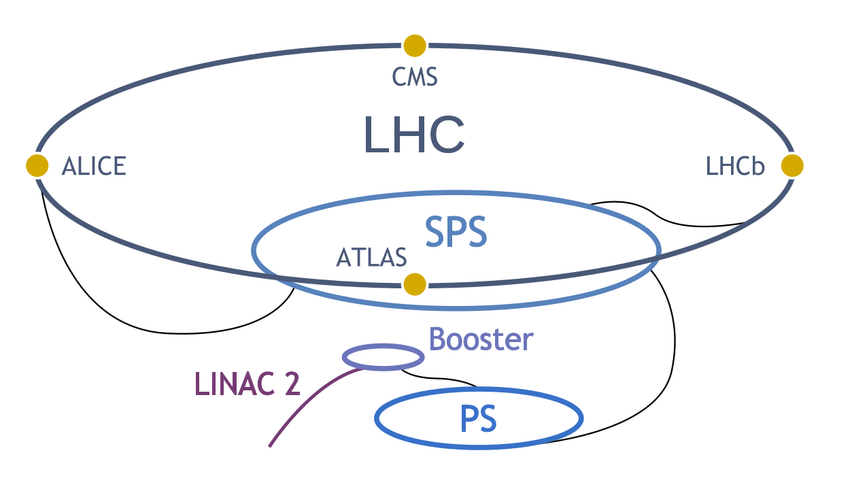
\includegraphics[width=\textwidth]{../ImmaginiTesi/LHC.png} 
  \end{minipage}
  \hfill 
  \begin{minipage}[b]{0.56\textwidth}
      \centering
      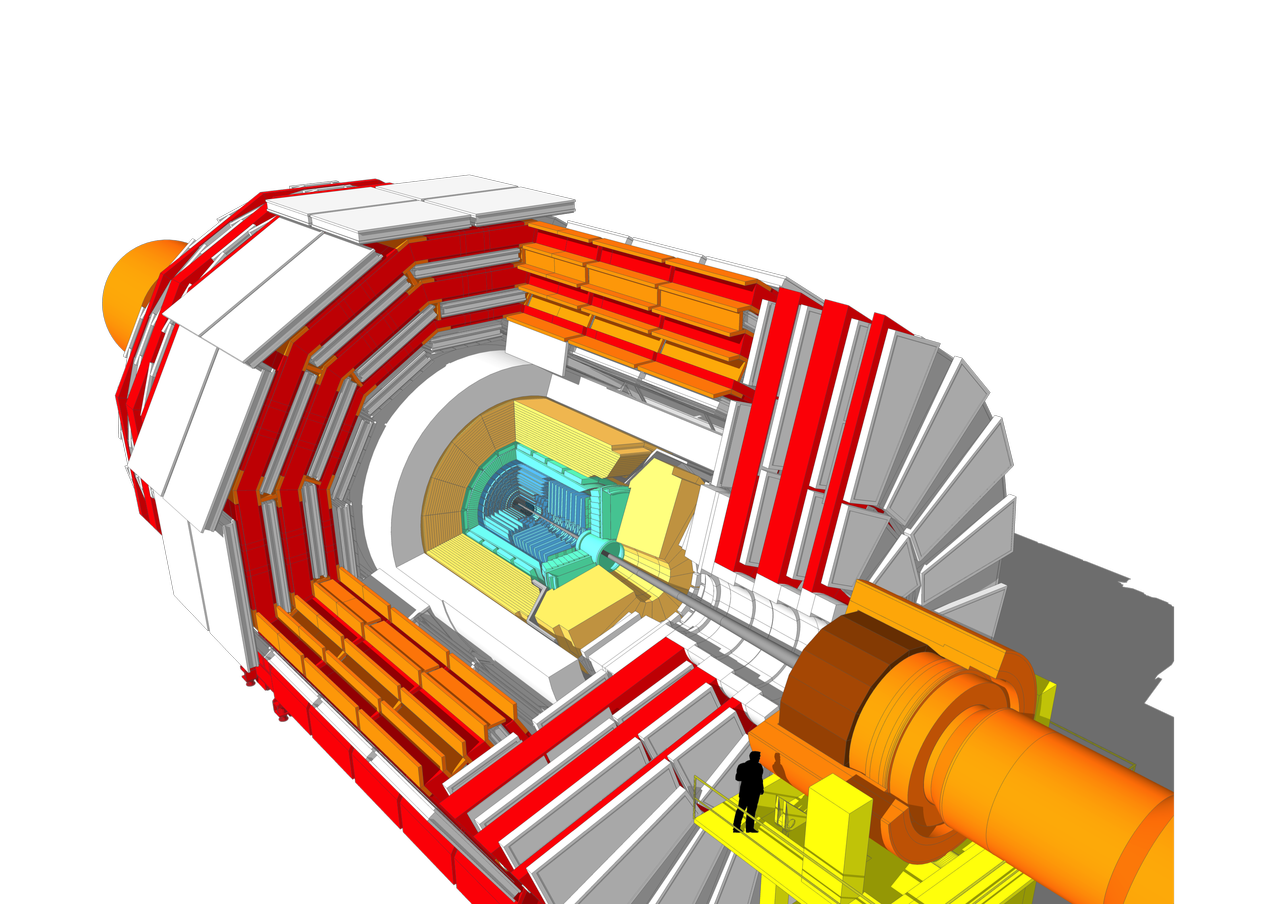
\includegraphics[width=\textwidth]{../ImmaginiTesi/CMS.png} 
  \end{minipage}
  \caption{Struttura dell'LHC e dei suoi rivelatori nei punti di interazione (sinistra), CMS (destra)}
  \label{fig:LHC-CMS}
\end{figure}


Prima di essere immessi in LHC, pacchetti formati da $1.1 \times 10^{11}$ protoni, subiscono varie fasi di accelerazione: inizialmente ad opera dell' acceleratore lineare Linac, poi dal Proton Synchrotron Booster (PSB), quindi dal Proton Synchrotron (PS) e infine dal Super Proton Synchrotron (SPS), dove vengono iniettati in LHC con una energia di 450 GeV. Circolando in due condotti differenti in direzioni opposte, i protoni vengono accelerati fino a 7 TeV collidendo frontalmente nei punti di interazione, (IP), con una energia nel centro di massa $\sqrt{s} \approx 14$ TeV. Come mostrato in figura \ref{fig:LHC-CMS}, i principali esperimenti di LHC sono ATLAS (IP1), Alice (IP2), CMS (IP5) e LHCb (IP8), nei rispettivi punti di interazione.


L'LHC alterna periodi di attività e di raccolta dati (\textit{Run}) con fasi di arresto in cui vengono effettuate opere di upgrade e di manutenzione generale per migliorare le prestazioni del collisore e dei rivelatori. Tra la Run 1, iniziata nel 2009 e finita nel 2013, e la Run 2, tra 2015 e 2018, il sistema di LHC ha subito un incremento dell'energia di collisione protone protone nel centro di massa da 8 a 14 TeV \cite{sirunyan2020performance}. Anche il sistema di acquisizione dati di CMS ha subito importanti miglioramenti (\textit{Phase 1}) rimpiazzando e potenziando hardware, elettronica e software per gestire il maggiore flusso di dati prodotto dalle collisioni ad alta energia. Tra i miglioramenti della Phase 1 vi è l'introduzione del \textit{Pixel Detector}, che permette una migliore gestione della maggiore luminosità istantanea di LHC \cite{Adam:2748381}. Ulteriori miglioramenti sono stati effettuati al sistema di trigger Level 1, L1T, di cui verrà discusso nel dettaglio nella Sezione \ref{sec:SistemaDiTrigger} \newline 
E' inoltre in programma a partire dal 2025, a seguito della Run 3, un ulteriore upgrade di LHC (\textit{Phase 2}) che porterà un incremento della luminosità istantanea fino a $5\times 10^{34}$ \Lumi, aumentando quindi il numero di collisioni medio per BX da 50 a 140 \cite{collaboration2021phase}. In contemporanea, al fine di sfruttare appieno l'incremento della luminosità di LHC della Phase 2 (noto come \textit{HL-LHC}, High Luminosity LHC), è previsto un ulteriore upgrade del sistema di detector di CMS, in particolare sul sistema di trigger Level 1.


\section{Compact Muon Solenoid}  
\label{sec:CMSDescrizione}

Locato nel punto di interazione IP5 in Cessy, Francia, il CMS è formato da un corpo cilindrico di 15 m di diametro e 21.6 m di lunghezza, per un peso di circa 14.000 tonnellate \cite{cms2008cms}. Sono vari gli ambiti di ricerca del rilevatore nel campo della fisica delle alte energie: dopo la scoperta del bosone di Higgs nel 2012 misurare le sue proprietà, attualmente compatibili con il modello standard, è diventato di fondamentale importanza. Ugualmente rilevante è anche la ricerca e lo studio di particelle esotiche e supersimmetriche con l'intento di esplorare Nuova Fisica oltre il modello standard. Al fine di identificare questi eventi rari è necessario un sistema di trigger molto performante \cite{sirunyan2020performance} e a questo scopo assume un'importanza centrale il nuovo sistema di trigger che verrà implementato nella \textit{Phase 2}, che permetterà quindi di osservare fenomeni esotici con una risoluzione migliore.

Di seguito una panoramica della struttura di CMS, dalle componenti più interne fino a quelle più esterne \cite{MasterThesisNicLai}(Figura \ref{fig:LHC-CMS}):

\begin{itemize}
  \item \textbf{Silicon Strip Tracker (SST):} Esegue una ricostruzione delle tracce e misurazione del momento trasverso di particelle originate da processi di interazione. 
  \item \textbf{Electromagnetic Calorimeter (ECAL):} Misure di energia di fotoni ed elettroni vengono eseguite grazie al tungstato di piombo (\si{PbWO_4}), materiale scintillante di cui è costituito l'ECAL.
  \item \textbf{Hadronic Calorimeter (HCAL):} Permette la misurazione delle energie degli adroni grazie al fenomeno della \textit{cascata adronica}, indotta dai materiali di cui è costituito l'HCAL e rivelata da materiali scintillatori plastici.
  \item \textbf{Solenoide superconduttore:} Formato dal superconduttore Niobio-Titanio (NbTi), produce un campo magnetico di intensità 3.8T nel nucleo. Un campo magnetico così elevato è fondamentale per permettere la curvatura di particelle cariche prodotte dalle collisioni, la cui rivelazione di tale curvatura permette di risalire a momento e carica delle stesse.
  \item \textbf{Camere muoniche:} Essendo i muoni particelle cariche elementari poco interagenti, il sistema di rilevazione muonico occupa una significativa porzione del volume di rilevatori di CMS. Suddiviso in tre regioni, \textit{barrel}, \textit{overlap} ed \textit{endcap}, il sistema delle camere muoniche copre il piano della pseudorapidità nel range $|\eta| < 2.4$, permettendo la rivelazione delle tracce di muoni usando tre diverse tecnologie: \textit{drift tube} (DT), \textit{resistive plate chamber} (RPC) e \textit{cathode strip chamber} (CSC) \cite{TheMuonProject} (Figura \ref{fig:SectorEtaView}).
\end{itemize}

L'origine del sistema di coordinate del Compact Muon Solenoid è centrato nel punto di collisione nominale dei fasci di protoni. L' asse \textit{y} è verticale, l'asse \textit{x} punta verso il centro di LHC e l'asse \textit{z}, segue la regola della mano destra, verso le montagne del Giura. L'angolo azimutale $\phi$ è misurato nel piano \textit{x-y} e l'angolo polare $\theta$ dall'asse \textit{z}. Sono di comune utilizzo variabili Lorentz invarianti nel contesto di condizioni ultrarelativistiche: per questo motivo la pseudorapidità, definita come $\eta = -\ln\left(\theta/2\right)$, è spesso preferita alla coordinata azimutale $\phi$. Per tanto il sistema di coordinate adottato a CMS è il sistema \textit{R-$\eta$-$\phi$} \cite{SearchHSCP}



\subsection{Camere muoniche:}

\begin{figure}[h]
  \centering
  \begin{minipage}[b]{0.48\textwidth}
      \centering
      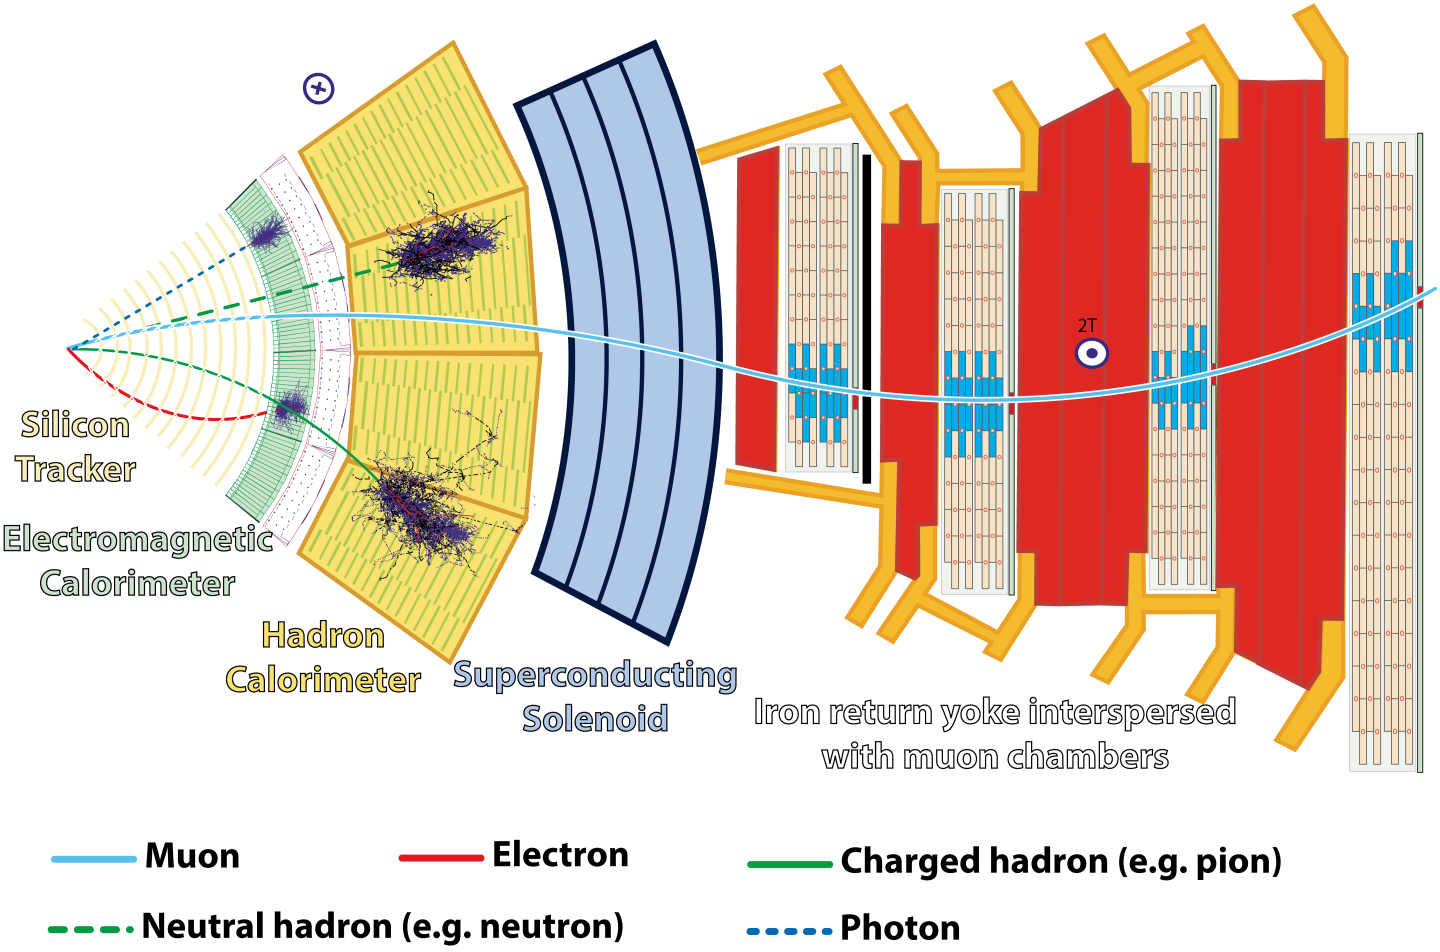
\includegraphics[width=\textwidth]{../ImmaginiTesi/CMS slice.png} 
  \end{minipage}
  \hfill 
  \begin{minipage}[b]{0.48\textwidth}
      \centering
      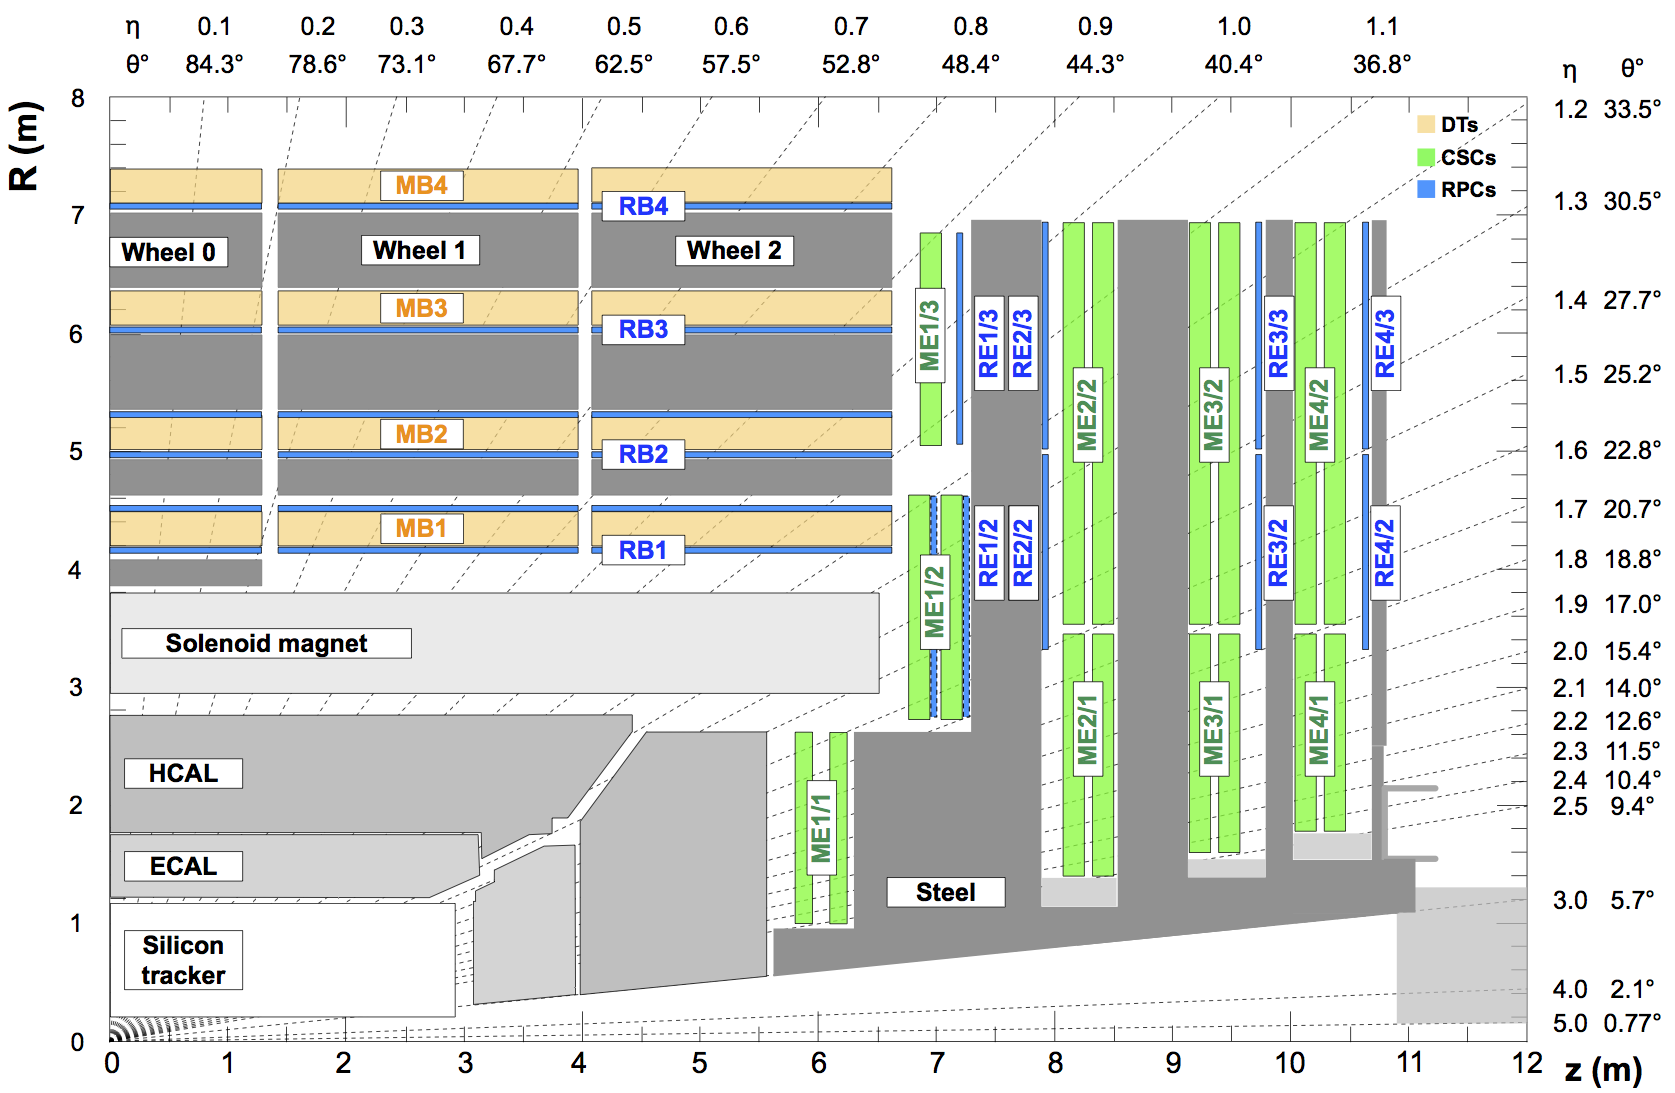
\includegraphics[width=\textwidth]{../ImmaginiTesi/CMSEtaView.png} 
  \end{minipage}
  \caption{Settore di CMS (sinistra), vista di CMS  nella variabile $\eta$ di CMS (destra)}
  \label{fig:SectorEtaView}
\end{figure}


L'alto rate di eventi di background a seguito di processi di interazione ad alta luminosità in LHC cela fenomeni interessanti: in questo contesto la rivelazione di muoni al CMS è uno strumento fondamentale per studiare tali fenomeni poiché i muoni sono particelle penetranti e per tanto meno soggette a interazioni con i materiali del rilevatore \cite{cms2008cms}. Il sistema muonico di CMS ha quindi tre funzioni: identificazione di muoni, misurazione del momento e trigger di muoni. Di seguito vengono descritti i sistemi di rilevazione dei muoni.




Come mostrato in figura \ref{fig:LHC-CMS} la regione di barrel, è formata da cinque ruote (\textit{wheel}), ognuna composta da dodici settori (\textit{sector}) e a loro volta da quattro stazioni concentriche (\textit{station}) interspaziate da una struttura di ferro nella quale è presente un campo magnetico di intensità circa 2T. Nella regione di barrel, dove gli eventi di background sono minimi, per la rivelazione di muoni vengono impiegati drift tube (DT), celle contenenti fili di acciaio inossidabile anodico disposte in modo adiacente una all'altra, separate da barre di alluminio che fungono da catodo: anodo e catodo operano ad un voltaggio rispettivamente di +3600V e -1200V. Quando un muone attraversa un DT la distanza tra la sua traiettoria e il filo di acciaio viene misurata a partire dal tempo di drift degli elettroni ionizzati che vengono attratti dal campo elettrico generato dalla differenza di potenziale tra catodo e anodo \cite{MasterThesisNicLai}. \newline
In totale il CMS contiene 250 DTs, disposti nella regione di barrel come in figura \ref{fig:SectorEtaView} ricoprendo la pseudorapidità nel range $|\eta| < 1.2$. \newline
Nelle regioni di endcap di CMS, dove il rate di muoni e livello di background è elevato ed il campo magnetico non uniforme, vengono impiegate CSCs che, grazie al loro design, permettono di ricavare precise informazioni spaziali e temporali sulle tracce di muoni nel range di pseudorapidità $0.9 < \eta < 2.4$. Le RPCs sono invece impiegate sia nella regione di barrel che nella regione di endcap, e assicurano una migliore misurazione del momento dei muoni grazie al loro rapido tempo di risposta \cite{MasterThesisNicLai}, \cite{cms2008cms}.


\subsection{Sistema di trigger:}
\label{sec:SistemaDiTrigger}

Non è possibile analizzare in tempo reale la mole di informazioni generata dal tasso di collisioni pari a 40MHz, per questo CMS è dotato di un sistema di trigger implementato come primo passo nella selezione di un processo fisico. 

Al fine di ridurre il volume di dati, mantenendo però gli eventi interessanti, il sistema di trigger si suddivide in due fasi: il \textit{Level 1 Trigger} (L1T) e l' \textit{High Level Trigger} (HLT) (figura \ref{fig:TriggerSystem}). 

Il Level 1 Trigger è implementato via hardware nel sistema di CMS, usando dispositivi programmabili come Field Programmable Gate Arrays (FPGA) e Lookup Table (LUTs) che, unendo informazioni del sistema muonico e del calorimetro, riducono il tasso di accetazione di eventi a 100KHz. Il processo di analisi preliminare e selezione deve avvenire rapidamente, in un tempo limite di 25 ns, per permettere a tutti gli eventi di essere analizzati dal trigger e ridurre quindi il numero di possibili eventi mancati; per questo il sistema di trigger L1 è si articola a sua volta in tre processi di analisi preliminare: \textit{locale}, \textit{regionale} e \textit{globale} \cite{MasterThesisNicLai}.
Il sistema di trigger quindi raccoglie le informazioni \textit{locali} dei calorimetri elettromagnetici e adronici (ECAL, HCAL) e informazioni sul sistema muonico (DTs, RPCs, CSCs). Le informazioni provenienti da processi locali, chiamate Trigger Primitive Generators (TPG) vengono combinate dai \textit{trigger regionali} che effettuano una classifica degli eventi sulla base di parametri come energia, momento trasverso e qualità. Quindi vengono passate al \textit{trigger globale} (GT) che determinerà se mantenere l'evento per una analisi ulteriore o se passarlo all' HLT.


Di fondamentale importanza in questo studio è il \textbf{sistema di Trigger Muonico} che permette la rilevazione e il tracciamento di muoni nelle tre regioni delle camere muoniche. Questo può essere suddiviso nelle tre regioni in $\eta$ descritte in sezione \ref{sec:CMSDescrizione} al fine di migliorare l'efficienza di ricostruzione dei muoni. Di seguito è riportata una più dettagliata descrizione di questo sistema \cite{sirunyan2020performance}.


Nella regione $\eta < 1.2$, le Trigger Primitives (TP) provenienti da DT e RPCs della stessa stazione vengono combinate dal TwinMux, un sistema introdotto con la \textit{Phase 1} che permette di ottenere una migliore risoluzione spaziale e temporale; i segnali combinati in uscita dal TwinMux sono chiamati \textit{superprimitives}, o stubs, ed ad ognuna viene assegnata una \textit{qualità}, che dipende dalle coordinate $\eta$ e $\phi$ dei TP in ingresso al TwinMux, e un \textit{angolo di curvatura interno} $\phi_b$. Le stubs vengono inviate quindi ai sistemi di tracciamento nella regione di barrel (\textit{Barrel Muon Track Finder}, BMTF) e nella regione di overlap (\textit{Overlap Muon Track Finder}, OMTF). Queste  ricostruiranno la traccia del muone usando le informazioni sulla qualità e sull'angolo di curvatura, ricavando anche informazioni riguardanti il momento trasverso $p_T$. \newline
Similmente nella regione di endcap ($1.2 < \eta < 2.4$) sono presenti delle schede CPPF (Concentrator Pre-Processor and Fan-out) che uniscono i segnali derivanti dalle Trigger Primitives delle RPCs della regione di endcap, ottenendo le coordinate $\phi$ ed $\eta$ che verranno mandate al sistema di tracciamento dell'endcap, \textit{Endcap Muon Track Finder} (EMTF). \newline
A questo punto fino a 108 tracce generate dai tre sistemi di tracker, corrispondenti a \textit{candidati muoni}, vengono inviate al Global Muon Trigger (GMT) che le classifica in base alla qualità, momento trasverso $p_T$ e provenienza (candidati muoni provenienti dalla regione di barrel possiedono infatti una qualità maggiore rispetto alla regione di endcap e overlap) e rimuovendo i duplicati. A questo punto fino ad 8 muoni vengono inviati al Global Trigger (GT). \newline
Infine il Global Trigger applica fino a 512 algoritmi di selezione ai muoni ricevuti dal GMT, decidendo se inviare un segnale di accettazione (Level 1 Accept) passando quindi l'evento all'HLT, riducendo l'output di rate di muoni a 100KHz \cite{CERNsummerSchool}.

L'HLT gioca un ruolo fondamentale nel filtrare ulteriormente gli eventi in uscita dal GT, mantenendo solamente quelli che hanno una importanza significativa e riducendo l'output a un rate di eventi pari a 1KHz . Al contrario del trigger L1, l'High Level Trigger è implementato via software e viene eseguito in una infrastruttura computazionale che conta 16000 CPU. \newline
Complessi algoritmi filtrano e selezionano gli eventi per soddisfare i requisiti di riduzione del volume di informazioni in entrata dell'HLT. I dati finali vengono quindi trasferiti nell'infrastruttura di storage del CERN \cite{MasterThesisNicLai}.


\begin{figure}[t]
  \centering
  \begin{minipage}[b]{0.40\textwidth}
      \centering
      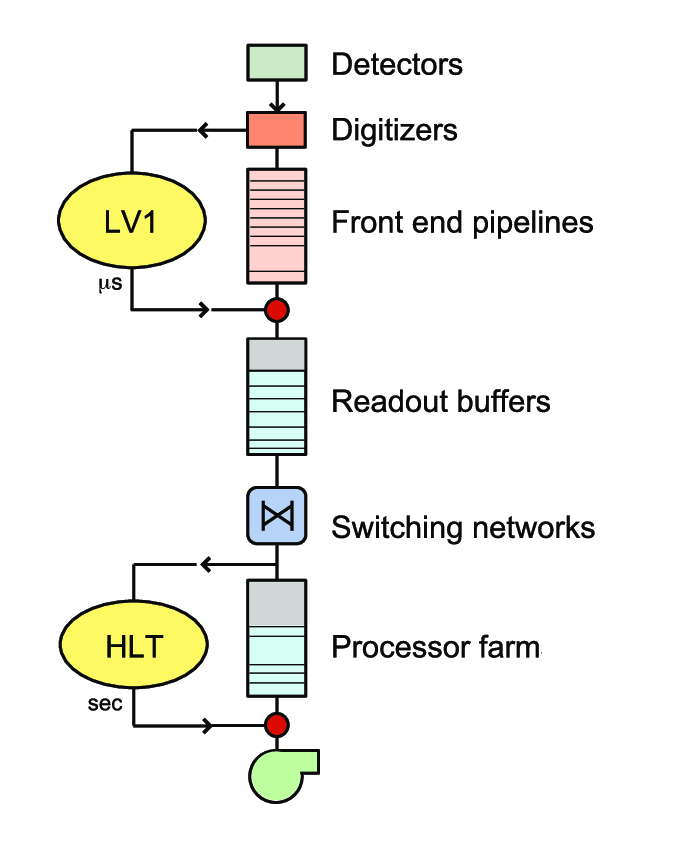
\includegraphics[width=\textwidth]{../ImmaginiTesi/TriggerSystem2.png} 
    \end{minipage}
    \hfill 
    \begin{minipage}[b]{0.48\textwidth}
      \centering
      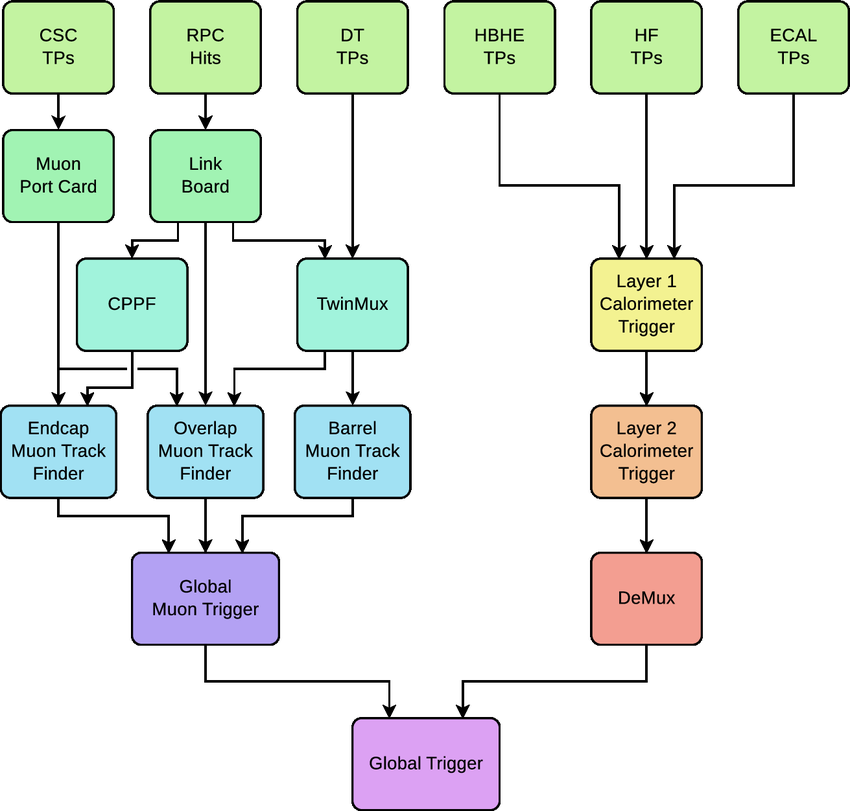
\includegraphics[width=\textwidth]{../ImmaginiTesi/TriggerSystem.png} 
  \end{minipage}
  \caption{}
  \label{fig:TriggerSystem}
\end{figure}


\section{Data Scouting e Phase 2}
\label{sec:DataScouting}


A seguito dell'interazione protone protone, il sistema di Trigger di CMS seleziona solamente una frazione degli eventi per una analisi più accurata, escludendone una porzione prevalente. Indubbiamente ciò introduce un \textit{pregiudizio} (bias) nella porzione di eventi minoritari che non vengono eliminati (vengono eliminati??) in quanto il sistema di Trigger filtra e seleziona dati che seguono leggi della fisica attualmente conosciute, possibilmente celando fenomeni sconosciuti e non teorizzati dal Modello Standard. \newline
In questo contesto il \textbf{ Data Scouting} (DS) è un approccio che si basa sulla analisi degli eventi direttamente nella catena di Trigger, estraendo e processando i dati online, aggirando il bias introdotto dal Trigger: evidentemente quindi più si esegue Scouting in superficie nella catena di trigger minore è il bias introdotto. L'approccio del Data Scouting si concentra sull'acquisizione di dati con un livello di risoluzione ridotto, consentendo però di raccogliere una statistica maggiore.

La tecnica di Data Scouting è stata utilizzata per la prima volta a livello dell High Level Trigger dove, per costruzione, solo 1 evento su 100 viene accettato. Qui è infatti possibile introdurre una nuova pipeline parallela al percorso standard dell'HLT che effettui Data Scouting su oggetti fisici che verrebbero possibilmente rigettati dal Trigger. La minore risoluzione di questi oggetti permetterebbe anche una analisi online e un immagazzinamento molto più efficace nel sistema di storage. 

Come già accennato in Sezione \ref{sec:LHC}, a seguito della Run 3, nel 2025, verranno effettuati importanti aggiornamenti alle componenti di LHC, permettendo di raggiungere un picco di luminosità istantanea pari a $5 \times 10^{34}$ \Lumi. Di conseguenza il CMS, ed in particolare il sistema di Trigger, deve essere a sua volta aggiornato per poter collezionare efficientemente il nuovo volume di informazioni di HL-LHC. Verranno implementati nuovi sensori che permetteranno di estendere la regione di raccolta dati fino a $|\eta| < 3.8$ e verranno modificati i sensori esistenti per avere una risoluzione migliore. Nel sistema di Trigger, verrà aumentato il rate di output massimo di eventi del L1T fino a 750KHz e quello di HLT fino a 7.5KHz. Ciò sarà possibile grazie all'utilizzo di nuovo hardware per l'analisi e per la ricostruzione delle tracce dei muoni usando GPU \cite{collaboration2021phase}.

\begin{figure}[t]
  \centering
  \begin{minipage}[b]{0.43\textwidth}
      \centering
      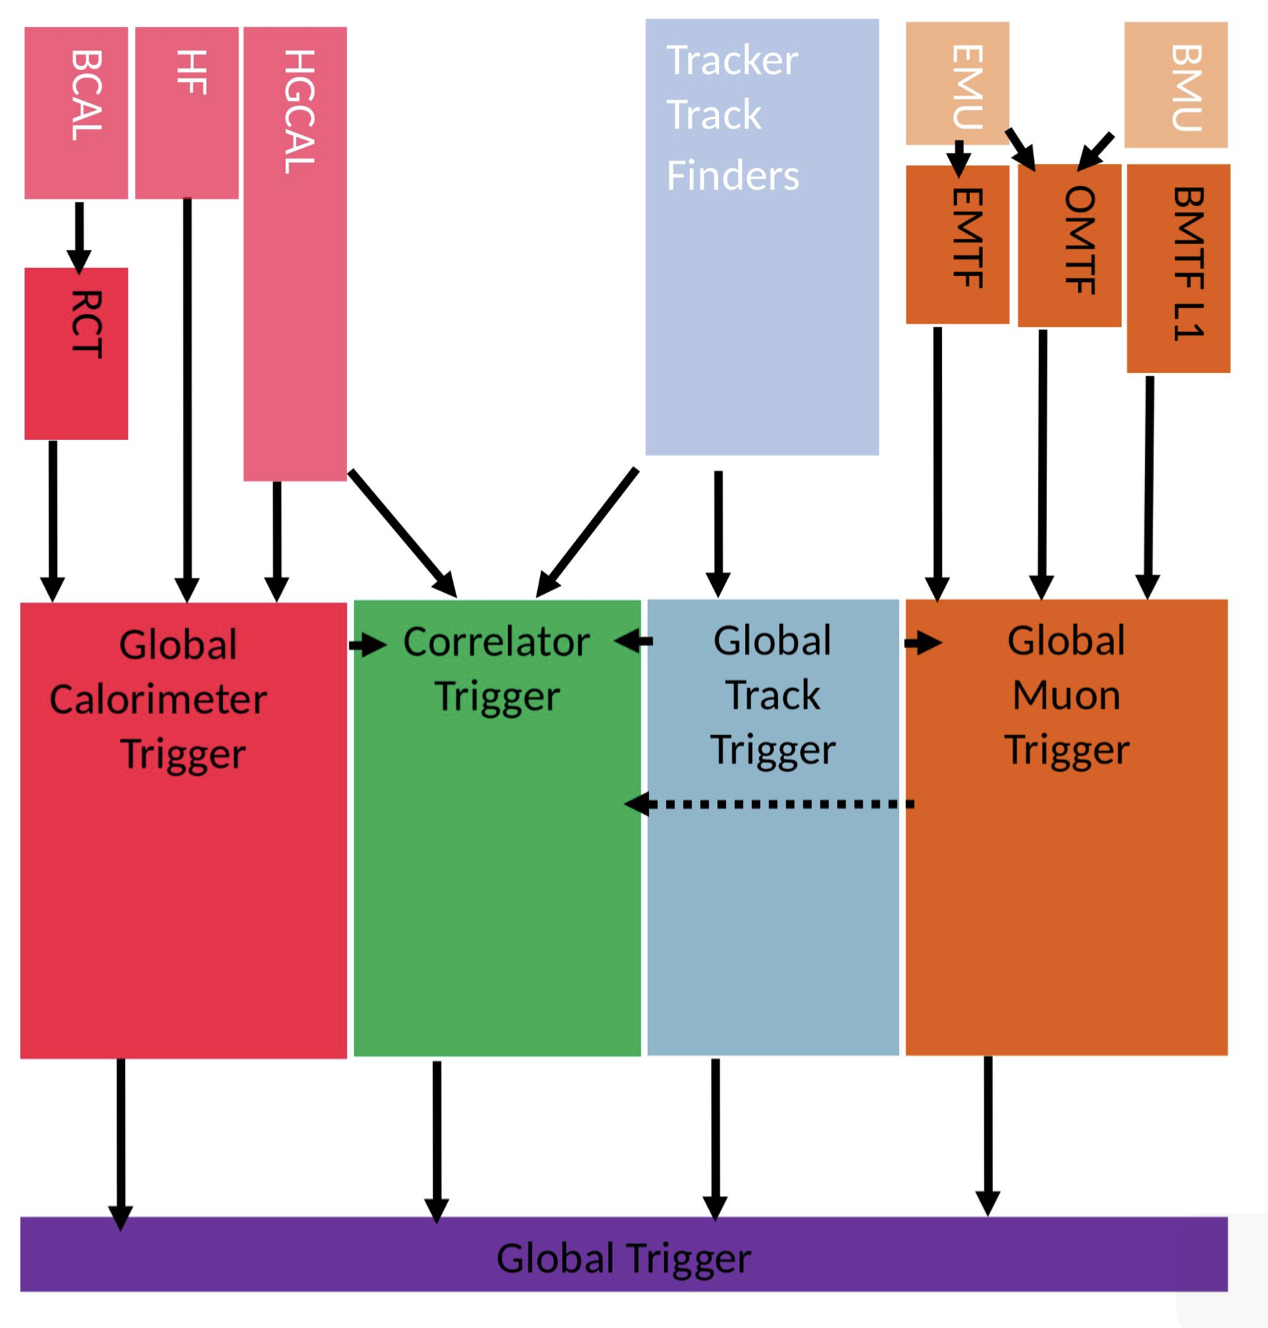
\includegraphics[width=\textwidth]{../ImmaginiTesi/Phase2.png} 
    \end{minipage}
    \hfill 
    \begin{minipage}[b]{0.48\textwidth}
      \centering
      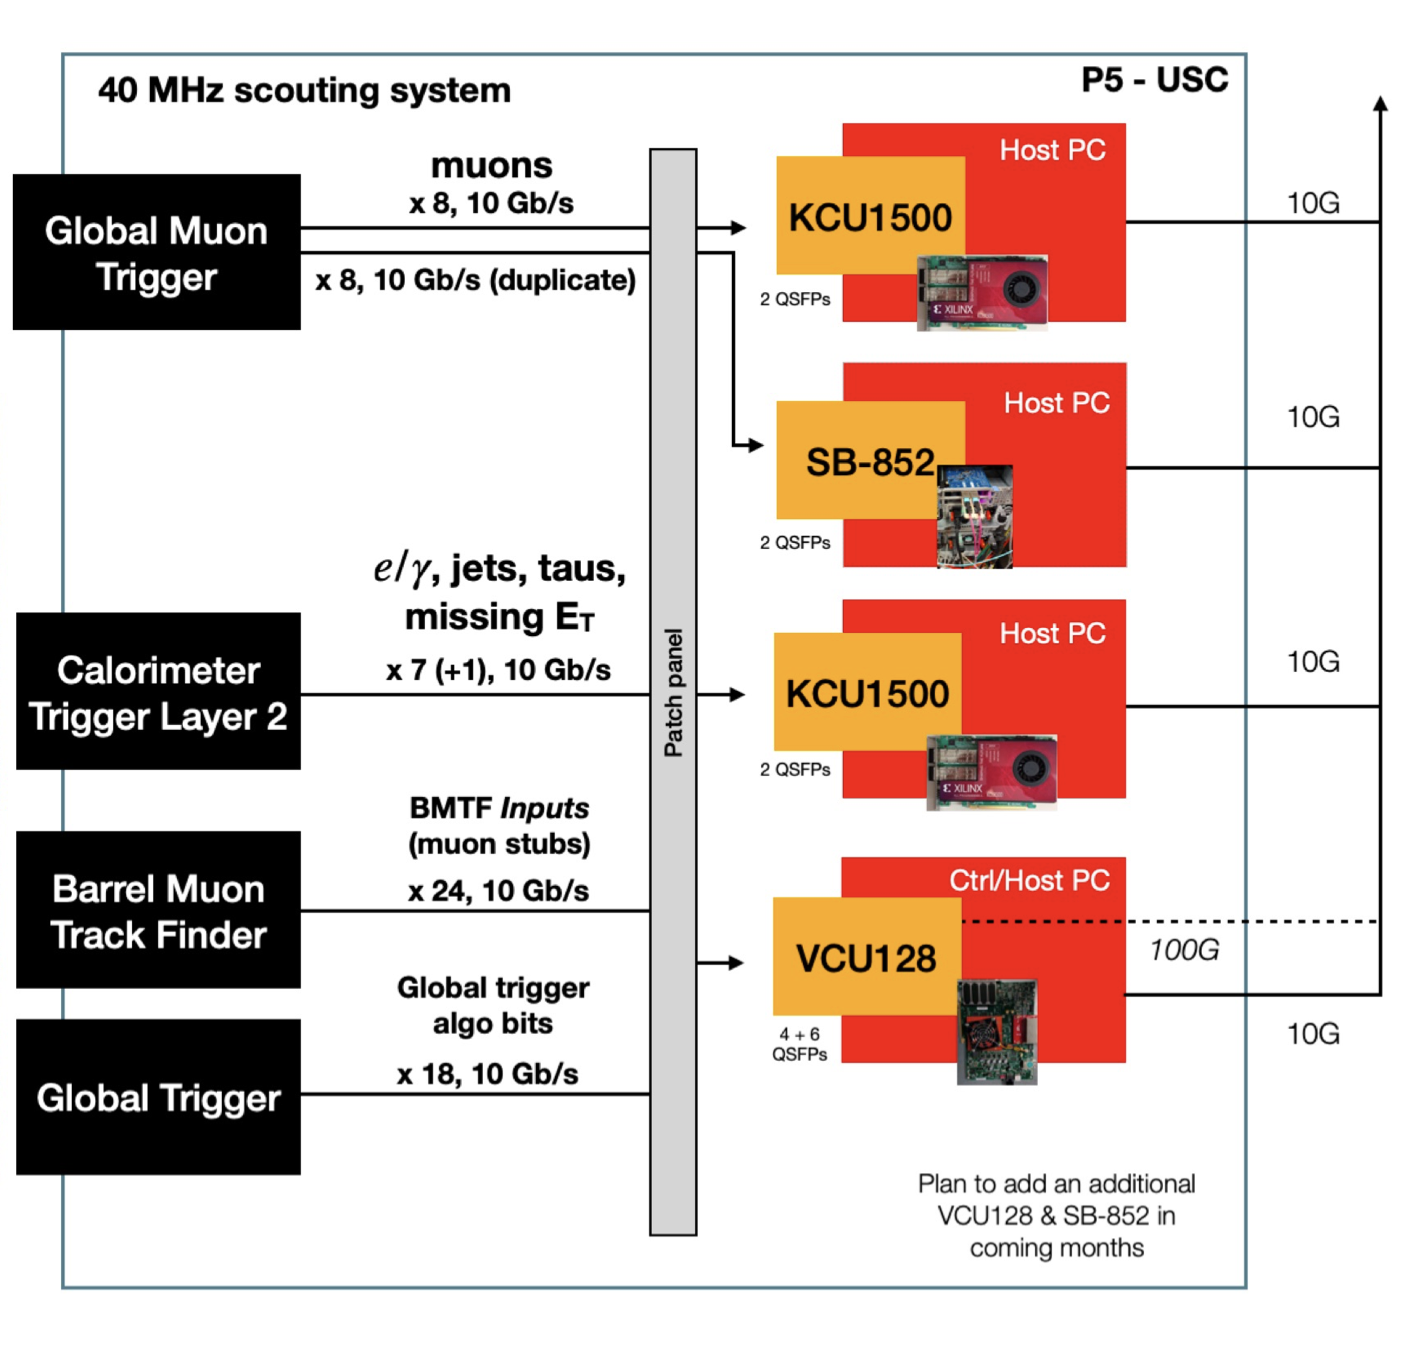
\includegraphics[width=\textwidth]{../ImmaginiTesi/DataScoutingRun3.png} 
  \end{minipage}
  \caption{}
  \label{fig:Scouting}
\end{figure}

Upgrade così importanti permetteranno di implementare la tecnica di Data Scouting nel Trigger Level 1 piuttosto che nell'HLT. Ciò offrirà una ancora più alta statistica di dati (relativamente) unbiased.\newline
Il sistema di Data Scouting nel L1T funzionerà in modo indipendente dal sistema di Trigger descritto in Sezione \ref{sec:SistemaDiTrigger}: verranno implementate schede FPGA dedicate che riceveranno i dati direttamente dagli output ottici delle schede di Trigger \cite{MasterThesisNicLai}.

Al fine di sperimentare l'utilizzo della tecnica di Data Scouting usando dati reali, durante la Run 3 un sistema apposito è stato implementato per raccogliere informazioni dai principali step di trigger del L1T. Più nel dettaglio il sistema raccoglie informazioni dal Barrel Muon Track Finder (BMTF), dal Calorimeter Trigger, dal Global Muon Trigger (GMT) e Global Trigger (GT) sfruttando una serie di schede FPGA diverse. In particolare, come mostrato in figura \ref{fig:Scouting} vengono impiegate due schede \textit{Xilinx KCU1500}, una scheda \textit{Micron SB852} e una \textit{Xilinx VCU128}. 


(MANCA UNA PARTE FINALE SUL DATA SCOUTING)




\section{Ricerca di Nuova Fisica al CMS}
\label{sec:NewPhysics}

Proposto inizialmente nel 1961 da Sheldon Glashow, e raffinato da Steven Weinberg e Abdus Salam nel 1968, il Modello Standard (SM) descrive tre interazioni fondamentali (Forte, Debole ed Elettromagnetica) che agiscono tra le particelle fondamentali che costituiscono la materia. Il beneficio di avere un frame così completo come il Modello Standard risiede nella capacità di prevedere il comportamento di particelle subatomiche conoscendo la struttura teorica alla base. Una delle maggiori conquiste dello SM è la scoperta del bosone di Higgs, teorizzato per la prima volta da Higgs nel 1964 e rilevato al CMS nel 2012. \newline
Nonostante negli ultimi 50 anni molte siano le conferme sperimentali del Modello Standard, ci sono fenomeni che non possono essere spiegati esaustivamente dal modello e questo suggerisce la presenza di fisica oltre il Modello Standard (Beyond Standard Model, BSM).

Diversi modelli di fisica oltre il Modello Standard suggeriscono la presenza di particelle cariche \textit{longeve} con masse di svariate centinaia di $GeV/c^2$, chiamate Heavy Stable Charged Particles (HSCPs). I modelli prevedono la presenza di due principali categorie di HSCPs \cite{Quertenmont:2010ota}: di tipo \textit{leptonico} o di tipo \textit{adronico}. Generalmente questi ultimi sono chiamati adroni-R (R-hadrons). \newline
Come gli adroni, gli adroni-R possono subire fenomeni di scattering da parte dei nuclei del materiale di cui sono formati i detector (scattering adronici). I modelli teorici suggeriscono però che la perdita di energia degli adroni-R a seguito scattering adronico sia molto ridotta e per tanto difficilmente rilevabile in calorimetri adronici; questo rende le HSPC particelle estremamente penetranti, ciò suggerisce che tali particelle si comportino come muoni e per tanto possano essere rilevate nelle camere muoniche. \newline
Essendo inoltre particelle cariche con un elevato tempo di vita medio (maggiore di 1ns) sono in grado di attraversare il detector prima di decadere, producendo ionizzazione nei detector.

Le principali firme sperimentali di HSCP sono quindi una anormale perdita di energia per unità di lunghezza $- \langle \frac{dE}{dx}\rangle$ e un maggiore tempo di volo (ToF) \cite{MasterThesisGioMoc}, riconducibili ad una velocità molto minore rispetto alla velocità della luce ($\beta < 1$). 

Prima della Phase 1 al CMS era implementato un sistema di trigger specifico per la ricerca di particelle massive con un lungo tempo di volo e una velocità molto minore della velocità della luce. Ciò era possibile in quanto, con una minore luminosità, vi era mediamente una collisione ogni 50ns. Con la Phase 1 e quindi con un aumento della luminosità istantanea e quindi un minore tempo di Bunch Crossing (uno ogni 25ns) il sistema di trigger per particelle esotiche è stato rimosso. 





\begin{comment}
  \renewcommand{\arraystretch}{1.35} % Aumenta lo spazio tra le righe
\begin{table}[h!]
  \centering
  \begin{tabular}{cccl}
  \toprule
  \textbf{Parameter} & \textbf{Bits} & \textbf{Range} & \textbf{Description} \\ \hline
  $\phi$            & 12  & [$-2048$, 2047]   & Relative position of a segment inside a sector \\ \hline
  $\phi_B$          & 10  & [$-512$, 511]     & Bending angle \\ \hline
  \textit{quality}  & 3   & [0, 7]            & Number of superlayers used to construct the stub \\ \hline
  $\eta$ hits       & 7   & "pattern"         & \begin{tabular}[c]{@{}l@{}} Each bit corresponds to one chamber area \\ 0 : no hit (less than 3 SL hits) \\ 1 : hit (3 or 4 SL hits) \end{tabular} \\ \hline
  $\eta$ quality    & 7   & "pattern"         & \begin{tabular}[c]{@{}l@{}} Each bit corresponds to one chamber area \\ 0 : 3 SL hits \\ 1 : 4 SL hits \end{tabular} \\ 
  \bottomrule
  \end{tabular}
  \caption{Parameter description}
\end{table}
\end{comment}